%==============================================================================
%== HCMUT DATN HK252 — Poster
%== Đề tài: Hoạch định chuyển động cho rô-bốt sử dụng tối ưu lồi
%==============================================================================

\documentclass[final]{beamer}
\usepackage[orientation=portrait,size=a0,
            scale=1.25
           ]{beamerposter}

\geometry{
  hmargin=2.5cm,
}

\usepackage[utf8]{inputenc}
\usepackage[vietnamese]{babel}
\usepackage[T5]{fontenc}

\usepackage{amsmath,amssymb}
\usepackage{booktabs}
\usepackage{subcaption}
\usepackage{tikz}
\usepackage{xcolor}
\usetikzlibrary{arrows.meta,positioning,shapes,backgrounds,calc}

\linespread{1.15}

%==The poster style============================================================
\usetheme{sharelatex}

% Custom colors aligned with theme
\definecolor{accentBlue}{RGB}{20,136,219}
\definecolor{deepBlue}{RGB}{3,43,145}
\definecolor{softGray}{RGB}{240,243,247}

%==Title, date and authors of the poster=======================================
\title
[HK252 -- DATN -- Hoạch định chuyển động cho rô-bốt sử dụng tối ưu lồi]
{
Hoạch định chuyển động cho rô-bốt sử dụng tối ưu lồi \\[0.4ex]
\normalsize \textit{Robot Motion Planning via Convex Optimization}
}

\author{
\textbf{MĐT:} HK252-DATN-028 \quad\textbar\quad
\textbf{GVHD:} PGS.\,TS.\,Lê Hồng Trang, ThS.\,Trương Quỳnh Chi \\
\textbf{SVTH:} Nguyễn Trần Đăng Khoa (2211635), Hồ Đăng Khoa (2211588)
}
\institute
[HCMUT]
{
Khoa Khoa học và Kỹ thuật Máy tính — Trường ĐH Bách Khoa, ĐHQG-HCM
}
\date{\today}


\begin{document}
\begin{frame}[t]
%==============================================================================
\begin{multicols}{2}
\justifying
%==============================================================================
%==The poster content==========================================================
%==============================================================================

\section{Đặt vấn đề}

\textbf{Bài toán:} Sinh quỹ đạo cho rô-bốt trong môi trường có vật cản,
đồng thời đảm bảo \emph{(i)} tránh va chạm, \emph{(ii)} trơn (liên tục $C^2$),
và \emph{(iii)} khả thi về mặt động lực học.

\medskip

\textbf{Thách thức cốt lõi:} không gian tự do $\mathcal{C}_{\mathrm{free}}$
là \emph{phi lồi}, khiến bài toán tổng quát thuộc lớp \emph{NP-hard}.

\medskip

\textbf{Hạn chế của các nhóm phương pháp hiện có:}
\begin{itemize}
    \item \textbf{Đồ thị (A\textsuperscript{*}, Dijkstra):} quỹ đạo zigzag,
    không khai thác cấu trúc liên tục của không gian.
    \item \textbf{Lấy mẫu (RRT, PRM):} kém tối ưu, khó nhúng ràng buộc
    \emph{kinodynamic}.
    \item \textbf{Tối ưu quỹ đạo trực tiếp (DMS):} dễ kẹt cực tiểu cục bộ
    khi có vật cản.
\end{itemize}

\medskip

% \textbf{Câu hỏi nghiên cứu:} \emph{Có thể kết hợp lựa chọn đường đi rời rạc
% với tối ưu quỹ đạo liên tục trong một khung tối ưu lồi/nguyên-hỗn hợp duy nhất?}


\section{Giải pháp \& Kiến trúc đề xuất}

% \subsection{Pipeline tổng thể}

\begin{figure}
\centering
\begin{tikzpicture}[
    node distance=10mm and 14mm,
    box/.style={
        rectangle, rounded corners=4pt, draw=deepBlue, line width=1.2pt,
        fill=softGray, text=deepBlue, font=\bfseries\small,
        align=center, minimum width=44mm, minimum height=14mm
    },
    branch/.style={
        rectangle, rounded corners=4pt, draw=accentBlue, line width=1.2pt,
        fill=accentBlue!12, text=deepBlue, font=\bfseries\small,
        align=center, minimum width=46mm, minimum height=18mm
    },
    output/.style={
        rectangle, rounded corners=4pt, draw=deepBlue, line width=1pt,
        fill=white, text=black!75, font=\small\itshape,
        align=center, minimum width=46mm, minimum height=12mm
    },
    arrow/.style={-{Stealth[length=4mm,width=3mm]}, line width=1.4pt, draw=deepBlue}
]

\node[box] (env)    {Môi trường có vật cản};
\node[box, below=of env] (decomp) {Phân hoạch không gian tự do\\\textit{\small ACD / IRIS / VCC}};
\node[box, below=of decomp] (graph)  {Đồ thị các vùng lồi\\$G=(V,E)$};

\node[branch, below left=15mm and 4mm of graph] (bez) {GCS-Bézier\\\small (MISOCP)};
\node[branch, below right=15mm and 4mm of graph] (dms) {GCS-DMS\\\small (MIOCP / MINLP)};

\node[output, below=10mm of bez] (outBez) {Quỹ đạo hình học\\\small tối ưu cận toàn cục};
\node[output, below=10mm of dms] (outDms) {Quỹ đạo động lực học\\\small khả thi cho rô-bốt};

\draw[arrow] (env) -- (decomp);
\draw[arrow] (decomp) -- (graph);
\draw[arrow] (graph.south) -| (bez.north);
\draw[arrow] (graph.south) -| (dms.north);
\draw[arrow] (bez) -- (outBez);
\draw[arrow] (dms) -- (outDms);

\end{tikzpicture}
\caption{Pipeline GCS tổng thể: phân hoạch không gian tự do, xây dựng đồ thị
các vùng lồi, rồi tối ưu quỹ đạo theo hai hướng bổ sung nhau.}
\label{fig:pipeline}
\end{figure}

\subsection{(A) GCS-Bézier --- tối ưu hình học}
\begin{figure}[H]
\centering
    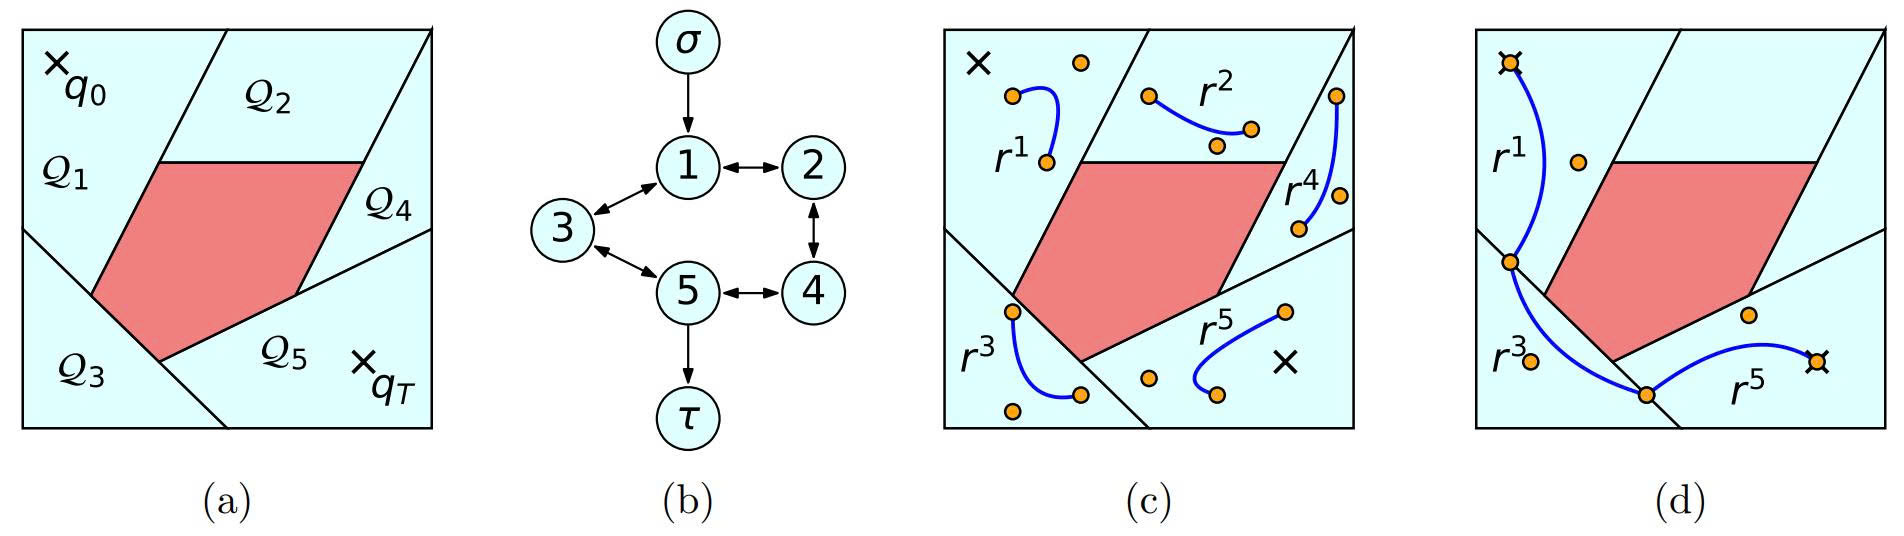
\includegraphics[width=\linewidth]{figures/pipeline.png}
    \caption{Quá trình quỹ đạo tối ưu.}
    \label{fig:maze}
\end{figure}
\begin{itemize}
    \item Tham số hoá quỹ đạo bằng \textbf{đường cong Bézier bậc $d$} trên từng vùng lồi.
    \item Tính chất bao lồi $\Rightarrow$ ràng buộc an toàn liên tục
    $\mathbf{x}(t)\in\mathcal{C}_{\mathrm{free}}$ trở thành ràng buộc tuyến tính
    trên các \emph{điểm điều khiển}.
    \item Áp dụng \textbf{nới lỏng phối cảnh} (perspective relaxation) + \textbf{RLT}:
    chuyển bài toán MICP về \textbf{MISOCP} giải hiệu quả bằng \texttt{Mosek}.
\end{itemize}


\subsection{(B) GCS-DMS --- tối ưu động lực học}

\begin{figure}[htbp]
    \centering

    \begin{subfigure}[t]{0.24\linewidth}
        \centering
        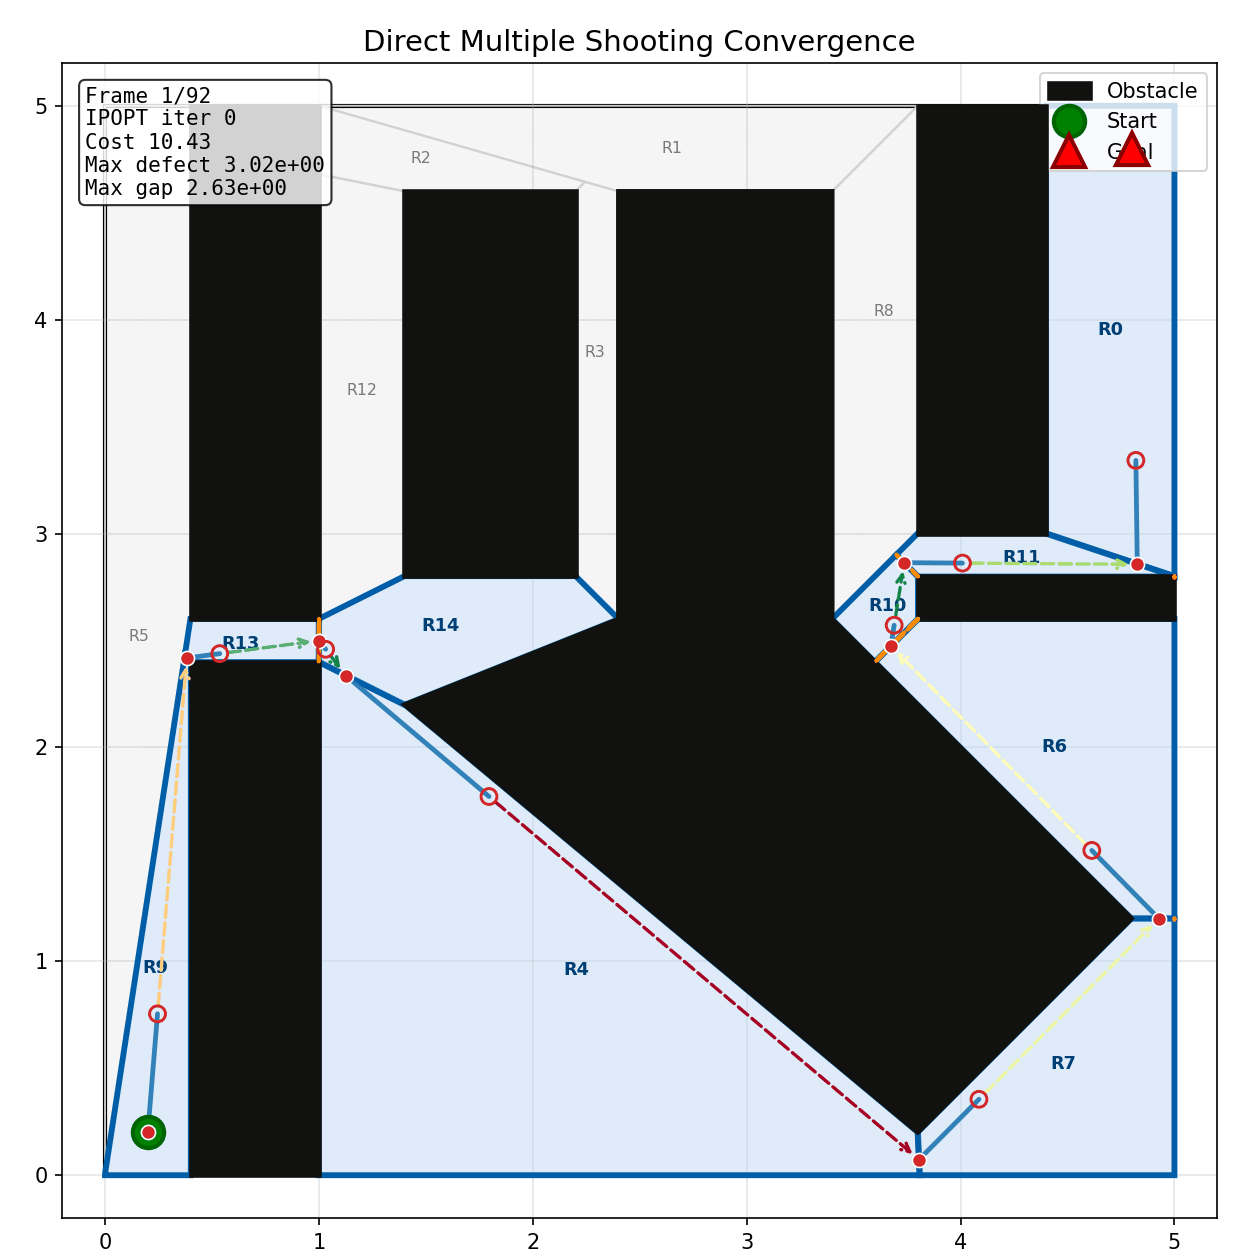
\includegraphics[width=\linewidth]{figures/conv_1.png}
    \end{subfigure}
    \hfill
    \begin{subfigure}[t]{0.24\linewidth}
        \centering
        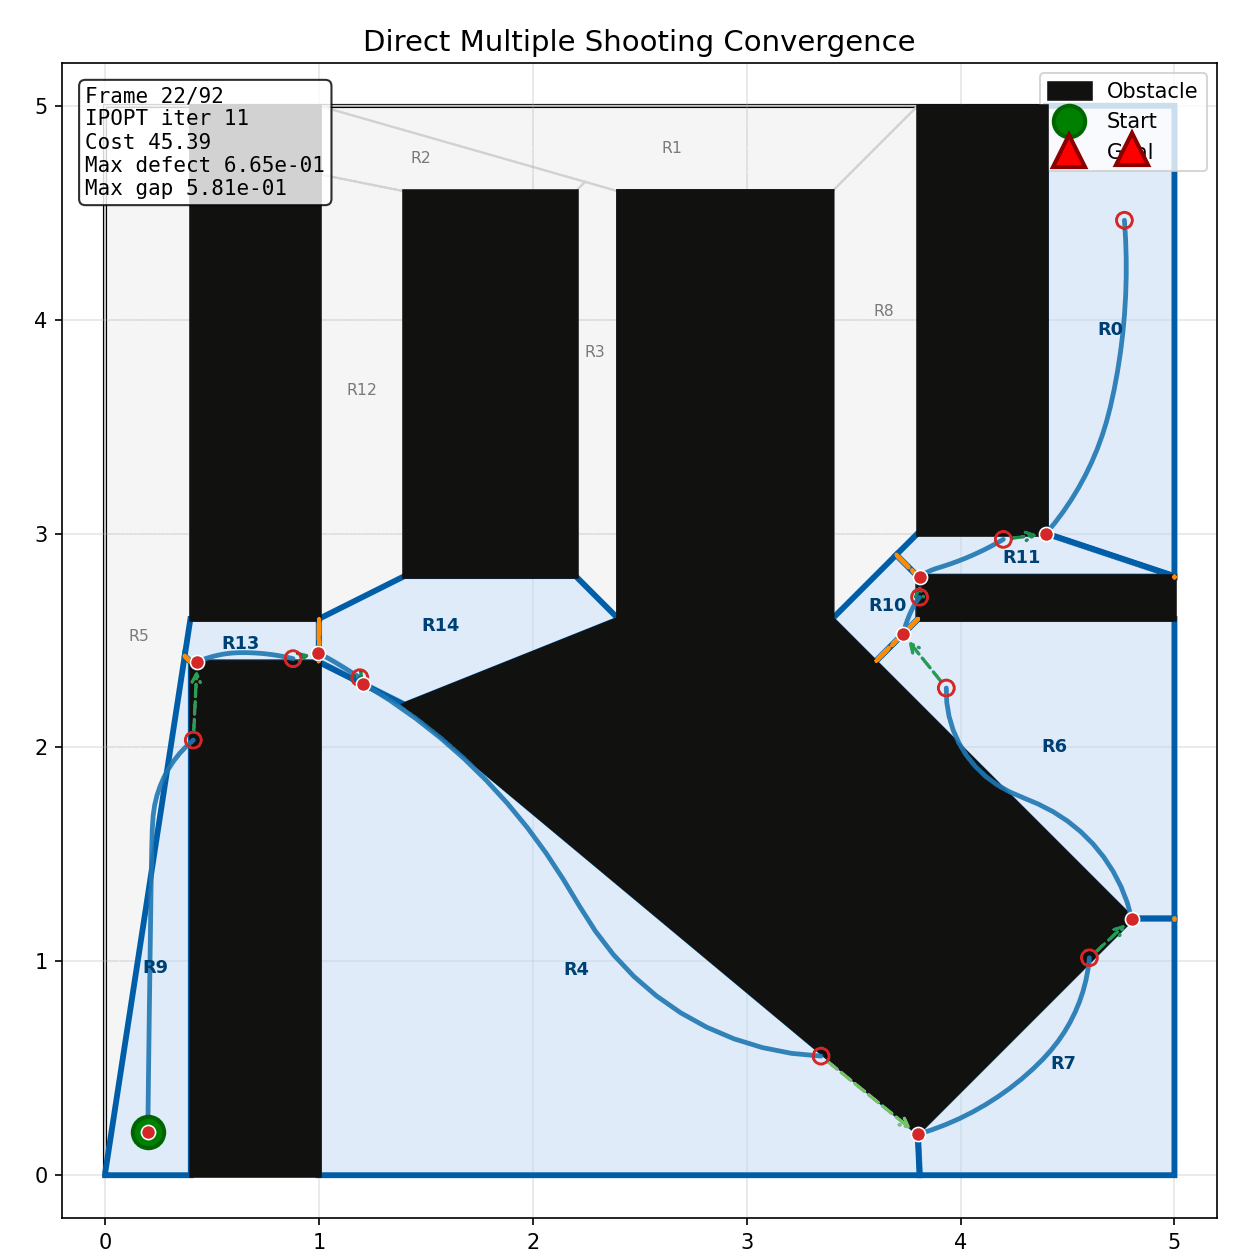
\includegraphics[width=\linewidth]{figures/conv_2.png}
    \end{subfigure}
    \hfill
    \begin{subfigure}[t]{0.24\linewidth}
        \centering
        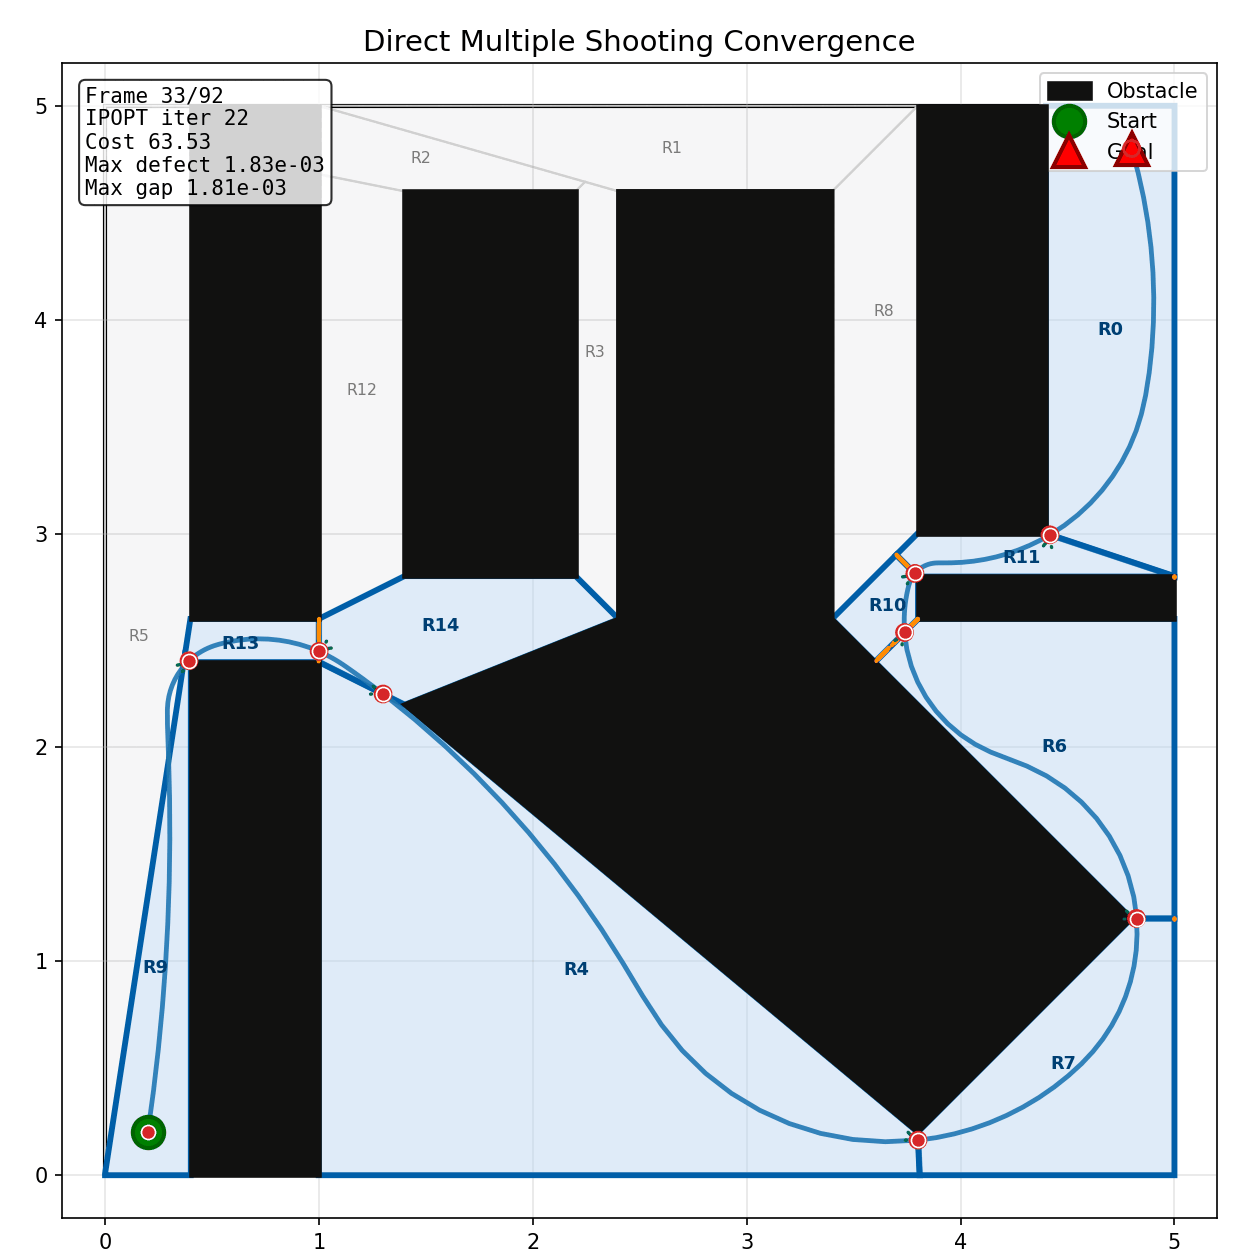
\includegraphics[width=\linewidth]{figures/conv_3.png}
    \end{subfigure}
    \hfill
    \begin{subfigure}[t]{0.24\linewidth}
        \centering
        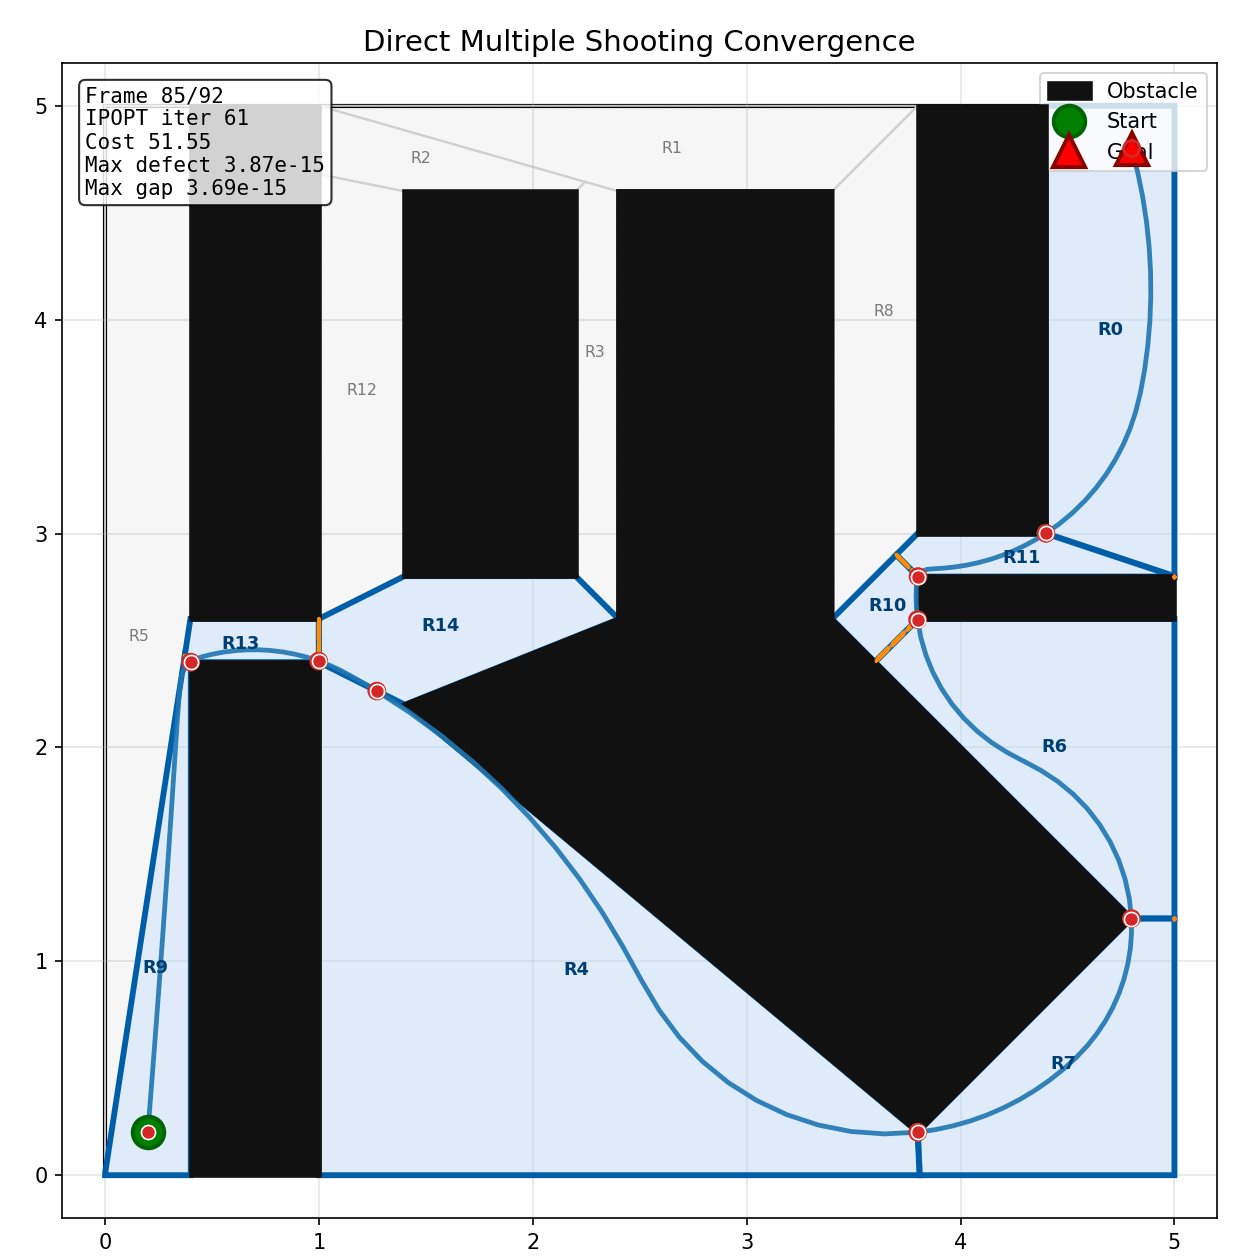
\includegraphics[width=\linewidth]{figures/conv_4.png}
    \end{subfigure}

    \caption{Quá trình hội tụ của DMS.}
    \label{fig:combined}
\end{figure}

\begin{itemize}
    \item Trên mỗi vùng lồi: \textbf{Direct Multiple Shooting} rời rạc hoá
    $\dot{\mathbf{x}}=f(\mathbf{x},\mathbf{u})$ thành các đoạn shooting.
    \item Ràng buộc an toàn xử lý theo 2 cơ chế: \textbf{lưới hữu hạn điểm}
    hoặc \textbf{hàm cản logarit} (log-barrier).
    \item Bài toán hợp nhất là \textbf{MIOCP} (liên tục) / \textbf{MINLP}
    (sau rời rạc hoá), giải bằng \texttt{CasADi}\,+\,\texttt{IPOPT}.
\end{itemize}

\subsection{Đóng góp chính}

\begin{enumerate}
    \item Tích hợp \textbf{3 phương pháp phân hoạch} (ACD, IRIS, VCC) vào cùng
    pipeline GCS và phân tích đánh đổi định lượng.
    \item Đề xuất \textbf{GCS-DMS với log-barrier}: mở rộng GCS sang lớp bài toán
    có động lực học phi tuyến.
    % \item Hệ thống thực nghiệm so sánh trên 3 môi trường có độ phức tạp
    % tăng dần.
\end{enumerate}


\section{Kết quả thực nghiệm}

% \subsection{So sánh phương pháp phân hoạch (môi trường 2D)}

% \begin{table}[H]
% \centering
% \footnotesize
% \caption{Tác động của thuật toán phân hoạch lên GCS-Bézier.}
% \label{tab:decomp}
% \renewcommand{\arraystretch}{1.4}
% \begin{tabular}{lccc}
% \toprule
% \textbf{Phân hoạch} & \textbf{Số vùng} & \textbf{Thời gian giải (s)} & \textbf{Path cost} \\
% \midrule
% Thủ công   & 12 &   3{,}90  & 27{,}88 \\
% \textbf{ACD}        & \textbf{15} & \textbf{4{,}31}  & \textbf{24{,}63} \\
% VCC        & 33 & 269{,}94 & 24{,}44 \\
% \bottomrule
% \end{tabular}
% \end{table}

% \textbf{Take-away:} ACD đạt cân bằng tốt nhất giữa số vùng và thời gian giải;
% VCC chỉ giảm path cost $\sim 1\%$ nhưng đắt gấp $\sim 64\times$ về thời gian.

\subsection{Mê cung 25\texttimes 25 (GCS-Bézier)}

\begin{figure}[H]
\centering
% \begin{minipage}{0.49\columnwidth}
    \centering
    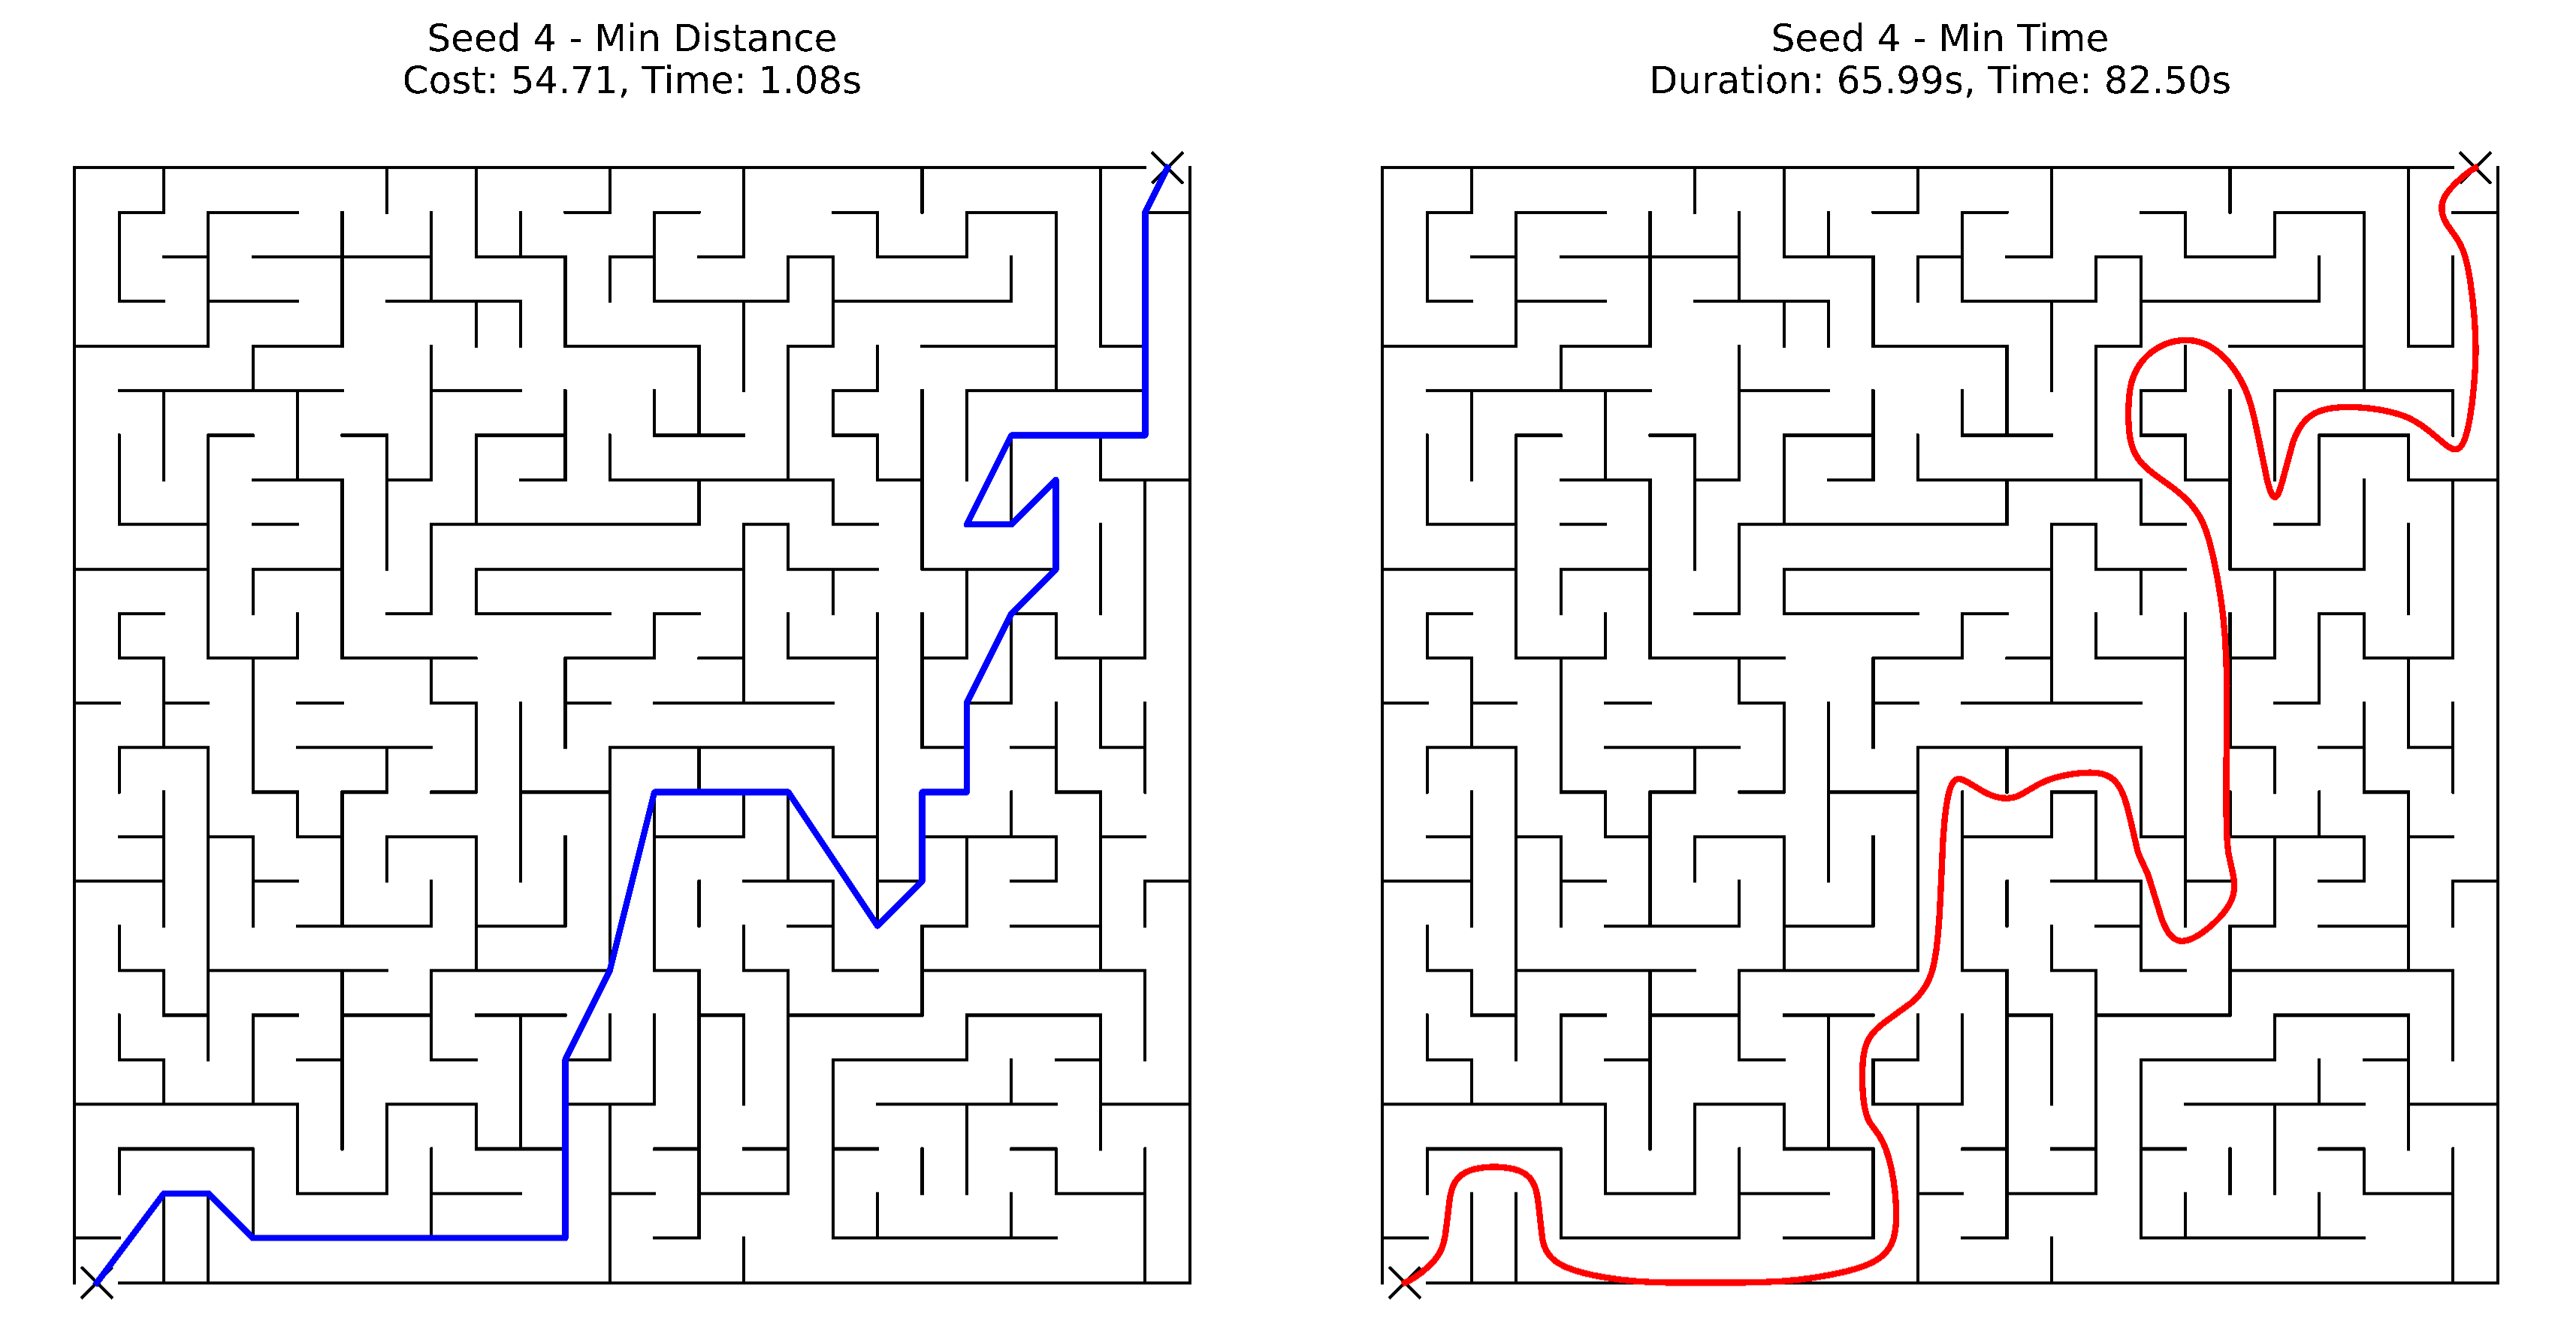
\includegraphics[width=0.7\linewidth]{figures/maze_traj.png}
    \caption{Quỹ đạo Bézier bậc 6, $C^2$, trên mê cung $25\times 25$.}
    \label{fig:maze}
% \end{minipage}
% \hfill
% \begin{minipage}{0.49\columnwidth}
%     \centering
%     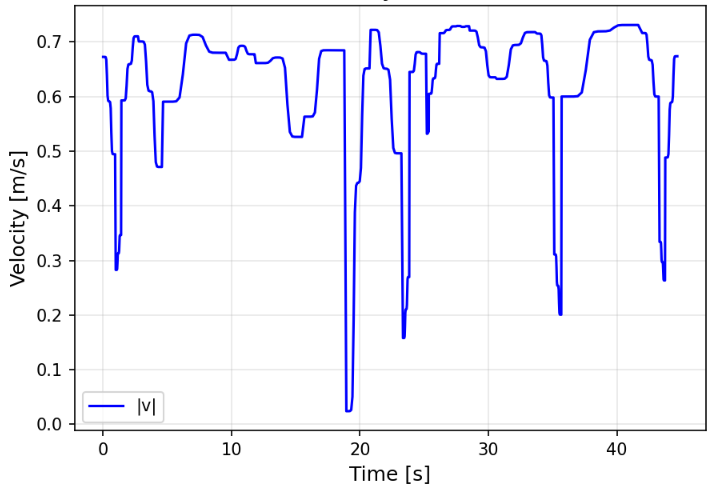
\includegraphics[width=\linewidth]{figures/dms_velocity.png}
%     \caption{Hồ sơ vận tốc Unicycle: giảm tốc tự nhiên ở đoạn cua hẹp.}
%     \label{fig:vel}
% \end{minipage}
\end{figure}

\begin{itemize}
    \item \textbf{Linear-GCS:} $1{,}28$ s, cost $71{,}88$ (chỉ tối ưu độ dài).
    \item \textbf{Bézier-GCS:} $85{,}22$ s, cost $88{,}03$ (thoả $C^2$, vận tốc, gia tốc).
    \item Relaxation cho ra \emph{xấp xỉ binary} trong mọi mẫu thử $\Rightarrow$ không cần rounding.
\end{itemize}

\subsection{GCS-DMS cho xe Unicycle nonholonomic}

\begin{figure}[H]
    \begin{subfigure}[t]{0.49\linewidth}
        \centering
        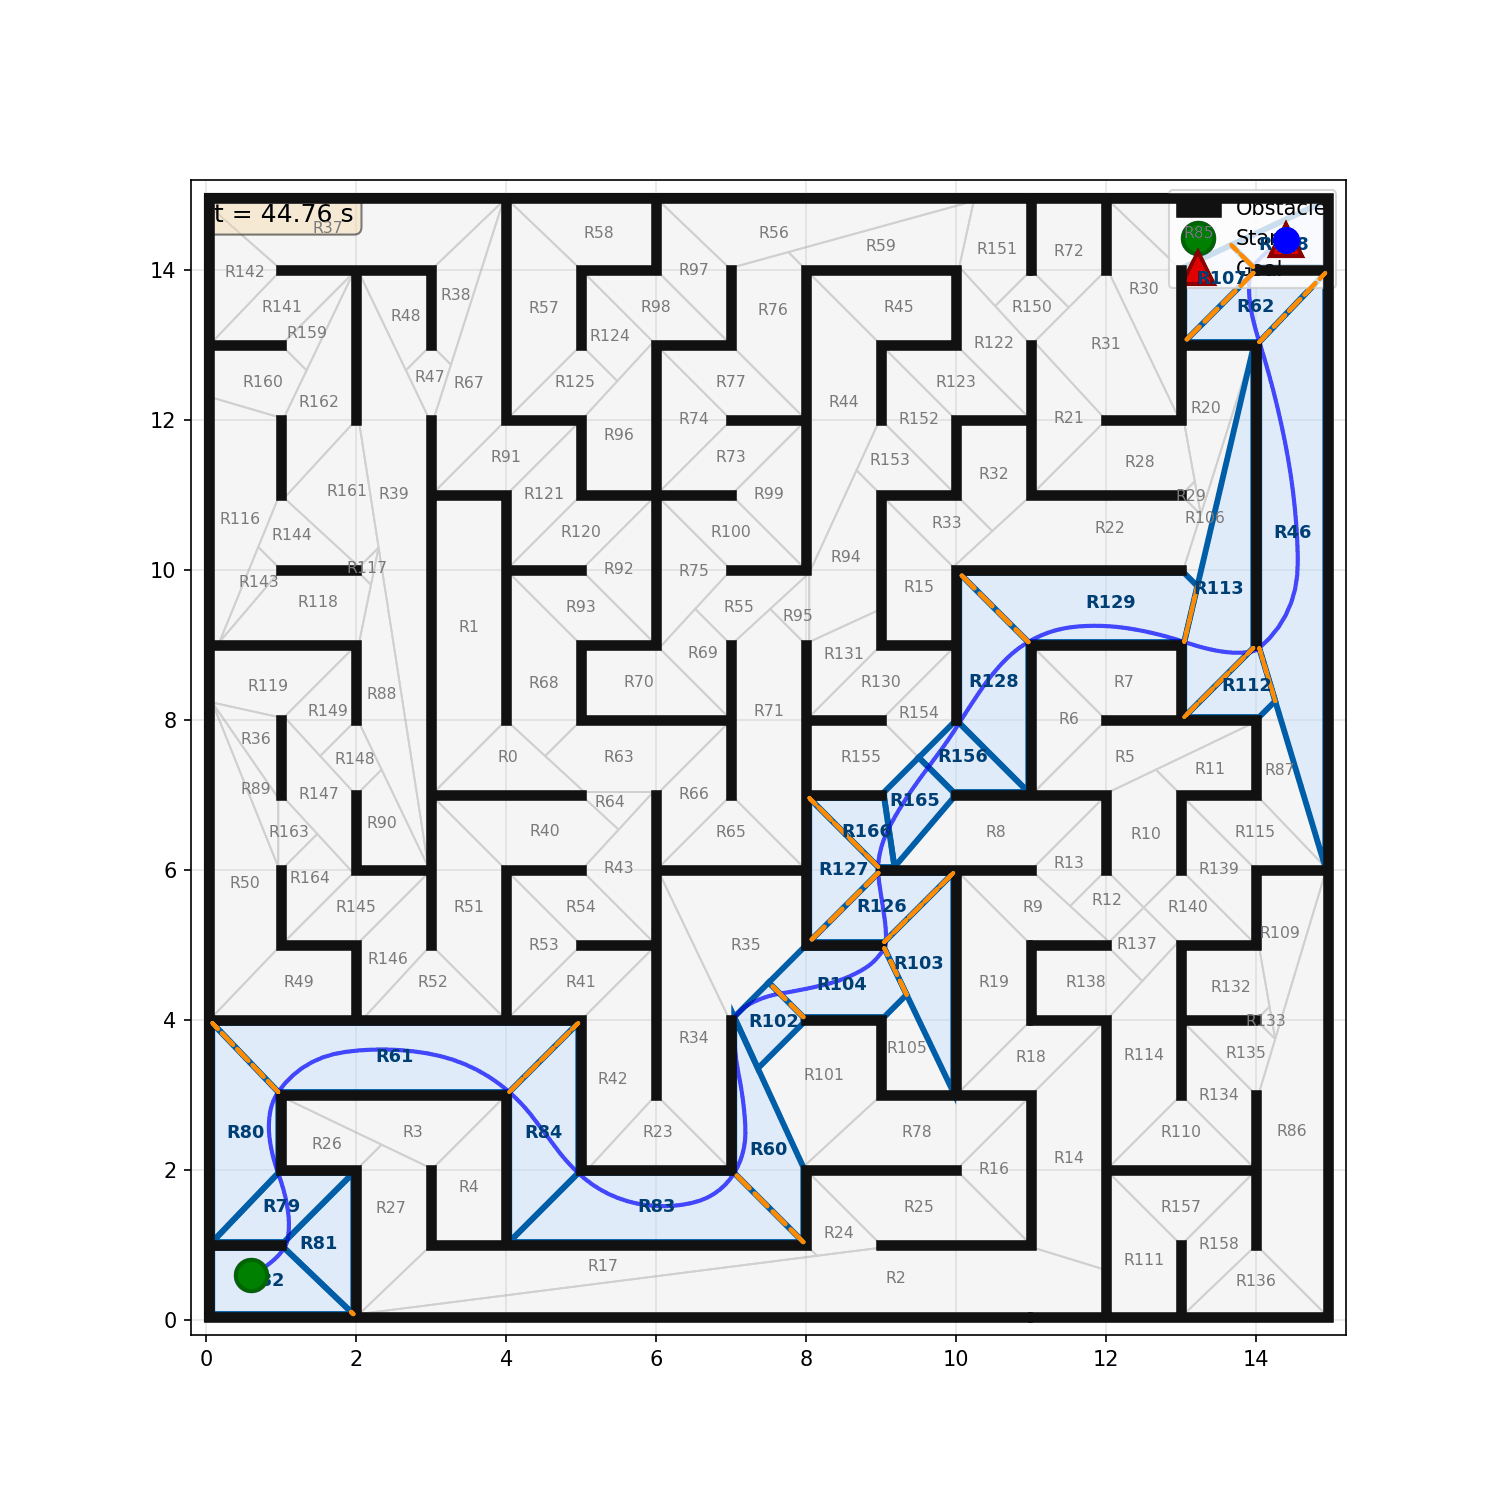
\includegraphics[width=\linewidth]{figures/dms_maze_seed4.png}
        \caption{Quỹ đạo GCS-DMS trên mê cung $15\times 15$.}
        \label{fig:dms_path}
    \end{subfigure}
    \hfill
    \centering
    \begin{subfigure}[t]{0.49\linewidth}
        \centering
        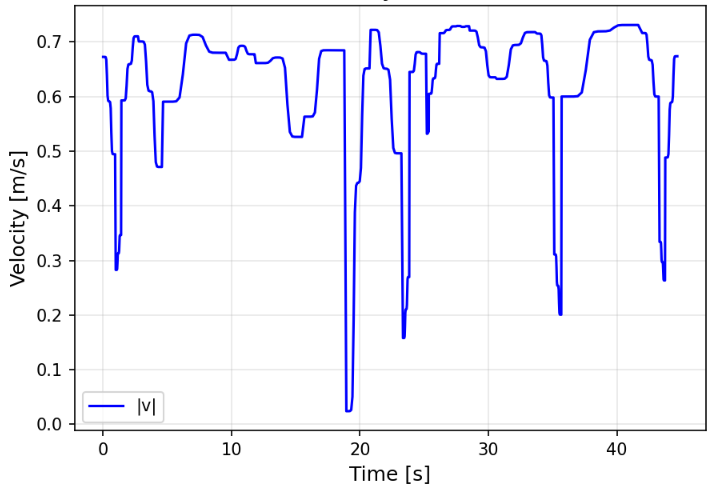
\includegraphics[width=\linewidth]{figures/dms_velocity.png}
        \caption{Hồ sơ vận tốc $|v|$ theo thời gian.}
        \label{fig:dms_vel}
    \end{subfigure}
    \caption{Kết quả GCS-DMS cho xe Unicycle.}
    \label{fig:dms_results}
\end{figure}



\begin{itemize}
    % \item Kiểm chứng trên 4 mê cung $15\times 15$ (seed 4, 17, 18, 20). Tất cả đều hội tụ.
    % \item Defect dynamics $\le 1{,}33\times 10^{-9}$, vi phạm hình học $\le 10^{-8}$
    % $\Rightarrow$ \textbf{quỹ đạo khả thi động lực học}.
    \item Vận tốc thẳng giảm tự nhiên ở các góc cua $\Rightarrow$ phù hợp giới hạn
    tốc độ góc lái của mô hình Unicycle.
\end{itemize}


\section{Kết luận \& Hướng phát triển}

\subsection{Kết luận}

\begin{itemize}
    \item Đã xây dựng pipeline GCS hoàn chỉnh: \emph{phân hoạch} $\to$ \emph{đồ thị vùng lồi}
    $\to$ \emph{tối ưu quỹ đạo} với hai hướng bổ sung nhau.
    \item \textbf{GCS-Bézier} ưu thế về tốc độ và cấu trúc lồi (MISOCP),
    phù hợp các bài toán hình học quy mô lớn.
    \item \textbf{GCS-DMS} mô hình hoá trực tiếp động lực học, đảm bảo quỹ đạo
    khả thi cho rô-bốt nonholonomic.
\end{itemize}

\subsection{Hướng phát triển}

\begin{itemize}
    \item Mở rộng sang \textbf{GCS không-thời gian} cho môi trường có vật cản di chuyển.
    \item Áp dụng \textbf{C-IRIS / IRIS-NP} cho cánh tay rô-bốt nhiều bậc tự do (7-DoF).
\end{itemize}


\subsection{Tài liệu tham khảo}

\begin{thebibliography}{9}
\footnotesize
\bibitem{Marcucci2023MP}
T. Marcucci \emph{et al.}, ``Motion Planning around Obstacles with Convex Optimization,'' \emph{Science Robotics}, 2023.

\bibitem{LienAmato2006}
J.\,M. Lien, N.\,M. Amato, ``Approximate Convex Decomposition of Polygons,'' \emph{CGTA}, 2006.

\bibitem{Diehl2006}
M. Diehl \emph{et al.}, ``Fast Direct Multiple Shooting Algorithms for Optimal Robot Control,'' Springer, 2006.
\end{thebibliography}

%==============================================================================
%==End of content==============================================================
%==============================================================================

\end{multicols}

%==============================================================================
\end{frame}
\end{document}
